% Classes de complexité
% =====================

\chapter{Classes de complexité}
\label{sec:classes_de_complexit_}
On va se ``limiter'' au problème de décision.

\begin{myrem}
	On ne se limite pas vraiment, car on
	peut facilement transformer un problème en un problème de décision.
\end{myrem}

\section{Réduction}
\label{sub:r_duction}

\paragraph{Objectif :} Déduire un algorithme pour un problème P' à partir d'un
algorithme P permet:
\begin{itemize}
	\item de prouver la calculabilité/non calculabilité
	\item d'analyser le degré de non-calculabilité
	\item de déduire la complexité
	\item d'analyser le degré de complexité
\end{itemize}

\begin{mydef}[Relation de réductibilité]
	$A \leq B$ : $A$ est réductible à $B$. Cette relation induit des classes
	d'équivalence. On peut comprendre ça comme $A$ est plus ``simple'' que $B$.
\end{mydef}

Il existe plusieurs méthodes de réduction qui ont des propriétés différentes.
Mais dans ce cours on va en étudier
que 3 :
\begin{itemize}
	\item réduction algorithmique
	\item réduction fonctionnelle
	\item réduction polynomiale
\end{itemize}

\begin{mydef}[$A$-complet]
	Soit $A$ une classe de problème, un problème $E$ est $A$-complet
	\textbf{par rapport} à une relation de réduction $\leq$ si
	\begin{enumerate}
		\item $E \in A$
		\item $\forall B \in A \ : \ B \leq E$
	\end{enumerate}
\end{mydef}

\begin{myrem}
	Le problème $E$ appartient à la classe de problème $A$ et
	est $A$-difficile.
\end{myrem}

\begin{mydef}[$A$-difficile]
	Soit $A$ une classe de problème, un problème $E$ est $A$-difficile
	\textbf{par rapport} à une relation de réduction $\leq$ si
	\begin{enumerate}
		\item $\forall B \in A \ : \ B \leq E$
	\end{enumerate}
\end{mydef}

\begin{myrem}
	N'importe quel problème de $A$ peut être réduit au problème $E$, mais $E$
	n'appartient pas nécessairement à $A$.
\end{myrem}


\subsection{Réduction algorithmique}
Ce type de réduction n'apporte aucune information au niveau de la complexité, car on
peut répéter autant de fois qu'on veut l'algorithme qui décide $B$. On peut aussi
faire un calcul avec une complexité très grande en plus d'utiliser $B$.

\begin{mydef}[Réduction algorithmique]
	Un ensemble $A$ est algorithmiquement réductible à un ensemble $B$
	($A\leq_a B$) si en supposant $B$ récursif, $A$ est récursif.
\end{mydef}

\begin{myrem}
	C'est à dire qu'en supposant qu'on connait un algorithme qui décide $B$, on
	peut construire un algorithme qui décide $A$.
\end{myrem}

\begin{myprop}
	Si $A \leq_a B$ et $B$ récursif, alors $A$ récursif (par définition)
\end{myprop}

\begin{myprop}
	Si $A \leq_a B$ et $A$ non récursif, alors $B$ non récursif (par définition)
\end{myprop}

\begin{myprop}
	$A \leq_a \stcomp{A}$
\end{myprop}

\begin{myprop}
	$A \leq_a B \ \iff \ \stcomp{A} \leq_a \stcomp{B}$
\end{myprop}

\begin{myprop}
	Si $A$ est récursif alors peu importe le $B$, $A \leq B$
\end{myprop}

\begin{myprop}
	Si $A \leq_a B$ et $B$ récursivement énumérable alors $A$ n'est
	\textbf{pas nécessairement récursivement énumérable}
\end{myprop}

\subsection{Réduction fonctionnelle}
Ce type de réduction n'apporte aucune information au niveau de la complexité,
car tout dépend de la complexité de la fonction $f$.

\begin{mydef}[Réduction fonctionnelle]
	Un ensemble $A$ est fonctionnellement réductible à un ensemble $B$
	($A\leq_f B$) s’il existe une fonction \textbf{totale calculable} $f$
	telle que
	\[ a\in A \ \iff \ f(a) \in B \]
\end{mydef}

\begin{myrem}
	Donc pour décider si $a\in A$ il suffit de calculer $f(a)$ et décider si
	$f(a) \in B$. Pour trouver une réduction fonctionnelle, il faut trouver
	une fonction qui transforme un problème de $A$ en un problème de $B$.
\end{myrem}

\begin{myprop}
	Si $A \leq_f B$ et $B$ récursif, alors $A$ récursif (par définition)
\end{myprop}

\begin{myprop}
	Si $A \leq_f B$ et $A$ non récursif, alors $B$ non récursif (par définition)
\end{myprop}

\begin{myprop}
	$A \leq_f B \ \iff \ \stcomp{A} \leq_f \stcomp{B}$
\end{myprop}

\begin{myprop}
	Si $A$ est récursif alors peu importe le $B$, $A \leq B$
\end{myprop}

\begin{myprop}
	Si $A \leq_f B$ et $B$ récursivement énumérable alors A est
	\textbf{nécessairement récursivement énumérable}
\end{myprop}

\begin{myprop}
	$A\leq_f B \Rightarrow A\leq_a B$ (Attention ce n'est pas toujours vrai
	dans l'autre sens)
\end{myprop}

\subsection{Différence entre $\leq_a$ et $\leq_f$}
La principale différence, c'est que $A \leq_a B$ est plus du point de vue de la
calculabilité. On s'intéresse au fait que ça soit possible, on peut utiliser
autant de fois que l'on veut le fait que $B$ soit récursif. \\
Alors que $A \leq_f B$ est plus du point de vue de la complexité. On est
obligé d'utiliser un certain schéma d'algorithme :

\begin{lstlisting}
input a
// some work
a2 := f(a)
// some work
if a2 in B then 1
else 0
\end{lstlisting}

On est donc limité à utiliser qu'une fois le test $f(a) \in B$ \textbf{en
	dernier lieu}.

\section{Modèles de calcul}
D'habitude, on utilise les machines de Turing pour avoir une définition précise
de la complexité. Mais c'est peu intuitif et on s'intéresse aux frontières. Or la
différence de complexité entre différents modèles est un facteur polynomial
(c'est une thèse) ce qui n'a pas d'influence sur les frontières.

\section{Classes de complexité}

\paragraph{Classes basées sur le modèle déterministe}
\begin{mydef}[DTIME(f)]
	Famille des ensembles récursifs pouvant être décidés par un programme
	Java de complexité temporelle $\mathcal{O}(f)$
\end{mydef}

\begin{mydef}[DSPACE(f)]
	Famille des ensembles récursifs pouvant être décidés par un programme
	Java de complexité spatiale $\mathcal{O}(f)$
\end{mydef}

\paragraph{Classes basées sur le modèle non déterministe}
\begin{mydef}[NTIME(f)]
	Famille des ensembles récursifs pouvant être décidés par un programme
	non déterministe Java de complexité temporelle $\mathcal{O}(f)$
\end{mydef}

\begin{myrem}
	On considère juste la complexité de la branche d'exécution la plus
	longue. Toutes les branches sont donc finies.
\end{myrem}

\begin{mydef}[NSPACE(f)]
	Famille des ensembles récursifs pouvant être décidés par un programme
	non déterministe Java de complexité spatiale $\mathcal{O}(f)$
\end{mydef}

\begin{mydef}[Classe P]
	\[ P = \mathop{\cup}_{i \geq 0} DTIME(n^i)\]
	Famille des ensembles récursifs pouvant être décidés par un programme
	Java de complexité temporelle polynomiale.
\end{mydef}

\begin{myrem}
	Les classes ne dépendent pas du modèle de calcul
\end{myrem}

\begin{mydef}[Classe NP]
	\[ NP = \mathop{\cup}_{i \geq 0} NTIME(n^i)\]
	Famille des ensembles récursifs pouvant être décidés par un programme
	Java non déterministe de complexité temporelle polynomiale.
\end{mydef}

\begin{myrem}
	Si on savait faire du non-déterminisme, on aurait une complexité polynomiale,
	mais pour le moment on ne peut que le simuler donc on a une complexité
	exponentielle.
\end{myrem}

\section{Relations entre les classes de complexité}
\label{sub:relations_entre_les_classes_de_complexit_}

\paragraph{Déterministe vs non-déterministe}
\begin{myprop}
	$A \in NTIME(f) \Rightarrow A \in DTIME(c^f)$ \\
	$f$ est la profondeur maximale de l'arbre. Si on simule le
	ND, alors on doit faire un bfs dans un arbre de profondeur $f$.
	$c$ est le facteur de branchement.
\end{myprop}

\begin{myprop}
	$A \in NSPACE(f) \Rightarrow A \in DSPACE(f^2)$ \\
	C'est une borne sur le nombre de nœuds d'un graphe de
	profondeur $f$. Théorème de Savitch.
\end{myprop}

\paragraph{Time vs Space}
\begin{myprop}
	$A \in DTIME(f) \Rightarrow A \in DSPACE(f)$ \\
	Le programme ne peut utiliser qu'au maximum un emplacement
	mémoire par instruction. Donc l'espace utilisé est limité par le
	nombre d'instructions.
\end{myprop}

\begin{myprop}
	$A \in NTIME(f) \Rightarrow A \in NSPACE(f)$ \\
	C'est la même chose que pour le cas déterministe (propriété précédente).
\end{myprop}

\begin{myprop}
	$A \in DSPACE(f) \Rightarrow A \in DTIME(c^f)$
    \begin{proof}
      On sait que le programme se termine car l'ensemble est récursif.
      La mémoire a un nombre exponentiel de configuration possible (stack, heap, program counter, ...).
      Si la complexité temporelle que le nombre de configuration possible,
      par le principe de tiroirs, on passe deux fois par la même configuration.
      On aura bouclé une fois.
      Mais comme la configuration détermine entièrement l'état du programme, on refera cette boucle une infinité de fois
      et le programme ne se terminera pas, ce qui contredit l'hypothèse.
    \end{proof}
\end{myprop}

\begin{myprop}
	$A \in NSPACE(f) \Rightarrow A \in NTIME(c^f)$ \\
	C'est la même chose que pour le cas déterministe (propriété précédente).
\end{myprop}

\paragraph{Hiérarchie de complexité}
On peut prouver qu'il existe pire qu'une complexité exponentielle.

\section{$NP$-complétude}
La question fondamentale de la complexité est la suivante :
\textbf{s'il existe un algorithme
non déterministe polynomial, existe-t-il un algorithme déterministe polynomial
résolvant ce même problème?}
 C'est-à-dire, est-ce que \textbf{$P = NP$?} On sait que $P
\subseteq NP$ mais on n'a pas encore montré si oui ou non $NP\subseteq P$.

\paragraph{} Pour démontrer ça, on essaye de montrer qu'un élément de $NP$, le
plus difficile, est dans $P$. On choisit un élément qui soit $NP$-complet par
rapport à une relation de réduction. Ainsi, si on y arrive, ça implique que
tous les autres éléments de $NP$ sont dans $P$ aussi.

\paragraph{} La question est maintenant de choisir la relation de réduction.
Les 2 relations de réduction définies précédemment ne suffisent pas. Ces
réductions ne permettent pas d'affirmer quelque chose sur la complexité. On
introduit donc une nouvelle réduction, la réduction polynomiale.

\begin{mydef}[Réduction polynomiale]
	Un ensemble $A$ est polynomialement réductible à un ensemble $B$, $A \leq
	_p B$ s’il existe une fonction \textbf{totale calculable} $f$ de
	\textbf{complexité temporelle polynomiale} telle que
	\[a\in A \ \Leftrightarrow \ f(a)\in B \]
\end{mydef}

\begin{myrem}
	On ajoute à la réduction fonctionnelle une contrainte de complexité
	sur la fonction $f$. Cette réduction nous permet donc de tirer des
	conclusions sur la complexité de $A$ connaissant la complexité de $B$.
\end{myrem}

\begin{myprop}
	\[ A \leq_p B \text{ et } B\in P \Rightarrow A\in P \]
	Ce qui est logique étant donné qu'on a la complexité de $f$ qui est
	polynomiale + la complexité de la décision de $B$ qui est aussi
	polynomiale.
\end{myprop}

\begin{myprop}
	\[ A \leq_p B \text{ et } B\in NP \Rightarrow A\in NP \]
	Ce qui est logique étant donné qu'on à la complexité de $f$ qui est
	polynomiale + la complexité de la décision de $B$ qui est non déterministe
	polynomiale.
\end{myprop}


\begin{mydef}[$NP$-complétude]
	Un problème $E$ est $NP$-complet (par rapport à $\leq_p$) si :
	\begin{enumerate}
		\item $E\in NP$
		\item $\forall B \in NP$ : $B\leq_p E$
	\end{enumerate}
\end{mydef}

\begin{myprop}
	Soit $E$ un ensemble $NP$-complet, \[ E \leq_p B \text{ \textbf{et} } B\in NP \Rightarrow \text{$B$ est $NP$-complet} \]
	Ce qui est logique puisque ça veut dire que $B$ est $NP$-difficile et dans
	$NP$.
\end{myprop}

En supposant $P \ne NP$, on peut représenter les différents classes de problèmes comme sur la figure \ref{fig:classe_prob}
\begin{figure}[h]
	\centering
	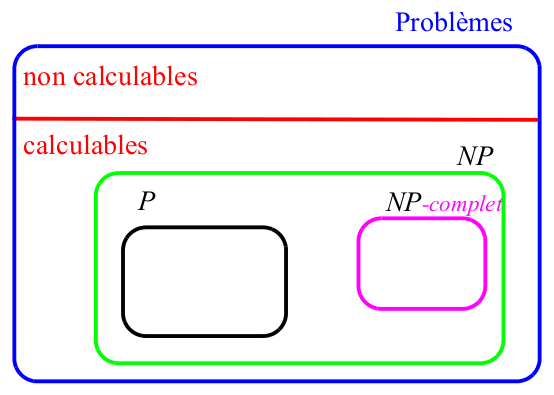
\includegraphics[width=0.6\textwidth]{Images/classes_prob.png}
	\caption{Classes de problèmes (en supposant $P \ne NP$)}
	\label{fig:classe_prob}
\end{figure}

\paragraph{} Nous allons désormais essayer de trouver des problèmes $NP$-complets et de
trouver des propriétés intéressantes sur $P$.

\subsection{Problème de décision}
On va définir différemment la classe $NP$. On va considérer des problèmes de
décision. Pour un ensemble $A$ cela consiste à dire si oui ou non une donnée $x$
appartient à $A$. On peut voir cela comme un prédicat. Par exemple $SAT(x)$ : la
formule $x$ est-elle satisfaisable?

\paragraph{Redéfinition de $P$ et $NP$} en problème de décision.

\begin{mydef}[Classe $P$]
	La classe $P$ est la classe des problèmes de décision pouvant être
	décidés par un algorithme polynomial.
\end{mydef}

\begin{mydef}[Classe $NP$]
	La classe $NP$ est la classe des problèmes de décision $A(x)$ pouvant
	s'exprimer sous la forme $\exists y \ B(x,y)$ tel que :
	\begin{itemize}
		\item $B(x,y) \in P$ (Il est donc facile de vérifier une
			solution)
		\item le domaine de $y$ est fini (taille polynomiale en $x$)
		       	et peut être généré, de manière non déterministe, en
			un temps polynomial
	\end{itemize}
\end{mydef}

\begin{myrem}
	On peut se représenter ça comme si le non-déterminisme permettait
       	de générer tous les $y$ ``en même temps'' ou
	que le non-déterminisme choisissait le bon $y$.
	Il est rapide de tester une solution, mais pas d'en trouver une.
\end{myrem}

\begin{mydef}[Calcul d'un problème $NP$]
	Pour décider $A(x)$
	\begin{enumerate}
		\item calculer $y$ (de manière non déterministe)
		\item déterminer $B(x,y)$
	\end{enumerate}
\end{mydef}

\section{Théorème de Cook : $SAT$ est $NP$-complet}
Pour pouvoir trouver des problèmes $NP$-complet en les réduisant par rapport à
un problème $NP$-complet, il faut trouver un premier problème $NP$-complet.
\paragraph{} On va montrer que $SAT$ est $NP$-complet en 2 parties :
\begin{enumerate}
	\item $SAT \in NP$
	\item $\forall B \in NP \ : \  B\leq_p SAT $
\end{enumerate}

\subsection{Le problème SAT}
Le problème $SAT(x)$ est de décider si la formule propositionnelle $x$ est
satisfaisable ou non. C'est-à-dire: est-ce que $x\in SAT$?

On définit l'ensemble $SAT$ comme l'ensemble des formules propositionnelles satisfaisables.


\begin{mydef}[Formule propositionnelle satisfaisable]
Soit $n$ variables $A_i$ booléennes, et une série de connecteurs logiques $\neg$ (non), $\wedge$ (et), $\lor$ (ou), $\Rightarrow$, $\Leftrightarrow$, (, ).
Une formule propositionnelle $x(A_1,...,A_n)$ est satisfaisable s'il existe des valeurs logiques (true ou false) pour les variables $A_1,...,A_n$ tel que $x(A_1,...,A_n)$ soit vraie.
\end{mydef}
\paragraph{} La longueur d'une formule $x$ est $O(n\log n)$, où $n$ est le nombre
d'occurrences des variables. Ça se justifie par le fait qu'en utilisant un codage
d'Huffman, le code pour une variable prendra $\log n$ (c'est important pour
définir la complexité du problème).
\begin{myexem} Soit les trois variables $A$, $B$ et $C$
	\[ x(A,B,C) = (\neg A \lor B) \wedge (B \lor C) \wedge (A \lor \neg C)\]
	$(\neg A \lor B)$, $(B \lor C)$ et $(A \lor \neg C)$ sont les trois clauses de notre formules. Elles ont chacune deux litéraux.
	La formule est ici satisfaite si $A=false$, $B=true$ et $C=false$. D'autres solutions sont possibles.
\end{myexem}

\subsection{$SAT \in NP$}
Il existe un programme ND polynomiale capable de décider si $x\in SAT$. On pose
que $m$ est le nombre de variables de $x$ et $n$ est le nombre d'occurrences de
variables ($m\leq x$). Étapes de l'algorithme avec leur complexité :
\begin{itemize}
	\item  Générer une séquence de $m$ valeurs logiques de façon
		non déterministe : $\mathcal{O}(m)$
	\item  Substituer les occurrences des variables par leur valeur :
	$\mathcal{O}(n
		\log n)$
	\item Évaluer l'expression : Complexité polynomiale par une technique
		de réduction.
\end{itemize}

\subsection{$\forall B \in NP \ : \  B\leq_p SAT $}
Comme $B \in NP$, on a une NDMT qui décide $B$ en un temps polynomial $p(n)$. On va
montrer qu'on sait transformer en un temps polynomial la NDMT par rapport à $n$
en une formule propositionnelle et que cette formule à une longueur qui dépend
de $p(n)$ ($\mathcal{O}(p(n))$ symboles). Ce qui prouve que $B \leq_p SAT$.

\paragraph{Idée de la transformation} Il me semble qu'on ne doit pas la connaitre
pour l'examen. Mais l'idée est de représenter le ruban comme un tableau de
variables booléennes (chaque ligne représente le ruban à un instant),
même chose pour les états, le curseur, l'alphabet,...


\section{Quelques problèmes $NP$-complets}
\begin{itemize}
	\item Problème du circuit hamiltonien HC (trouver un chemin qui passe
		une seule fois par tous les sommets)
	\item Problème du voyageur de commerce TS (trouver un chemin qui relie
		tous les sommets et de longueur $\leq B$)
	\item Chemin le plus long entre 2 sommets dans un graphe
	\item $3SAT$ (forme conjonctive avec 3 variables par clause)
	\item Programmation entière (simplexe)
	\item ...
\end{itemize}
